\documentclass[11pt]{article}
\usepackage[a4paper,margin=1in]{geometry}
\usepackage{amsmath,amssymb,amsthm}
\usepackage{graphicx}
\usepackage[round]{natbib}
\usepackage[hidelinks]{hyperref}
\usepackage{microtype}
\usepackage{enumitem}
\usepackage{algorithm}
\usepackage{algpseudocode}
\setlist{nosep,leftmargin=1.5em}
\usepackage{caption}
\captionsetup{font=small,labelfont=bf}

\newtheorem{theorem}{Theorem}
\newtheorem{lemma}{Lemma}
\newtheorem{proposition}{Proposition}
\newtheorem{corollary}{Corollary}
\theoremstyle{definition}
\newtheorem{question}{Question}
\newtheorem{hypothesis}{Hypothesis}

\newcommand{\Var}{\operatorname{Var}}
\newcommand{\E}{\mathbb{E}}
\newcommand{\Rn}{R_n}
\newcommand{\ADm}{\widehat{AD}_m}
\newcommand{\Om}{\widehat{O}_m}
\newcommand{\ADinf}{AD_\infty}

\title{\vspace{-1.4em}\textbf{From Estimation to Certification:\\ An Irreducible Floor in Partial Observation}\\[0.35em]
\normalsize Supplement to \emph{Bayesian Inference in Random Transposition Shuffles}}
\author{Mihika Singhania}
\date{}

\begin{document}
\maketitle
\vspace{-2em}

\begin{abstract}\noindent\small
The parent paper establishes that the global average displacement of a random-transposition shuffle can be estimated from a uniform sample of $m$ of its $n$ cards with relative uncertainty $1/\sqrt{2m}$, independent of $n$. We recast that estimation result as a \emph{certification} problem and identify the quantity that governs it. Expanding the estimator variance by the law of total variance separates a sampling term, of order $1/m$, from an $m$-independent floor equal to the observable's equilibrium variance. This floor is a strict lower bound on relative error, and whether it vanishes with system size is determined by the susceptibility $\chi_n=n\,\Var_\nu(O)$, with dividing line $\chi_n=O(1)$. We evaluate the floor exactly for the shuffle (constant $2/5$), give a size-free sufficiency condition, and report a measured consequence at the two-dimensional Ising critical point, where the energy is certifiable and the order parameter is not. We then state the open problems and a proposed algorithm for estimating the floor from a single realisation.
\end{abstract}

\section{Motivation and Problem Formulation}
Let a finite system have $n$ components, stationary law $\nu$, and bounded per-component contributions $D_i(x)\in[0,B]$ in configuration $x$. The intensive observable is $O(x)=\tfrac1n\sum_{i=1}^n D_i(x)$, with equilibrium mean $O_\infty=\E_\nu[O]$. An observer draws a uniform subset $S\subseteq[n]$ of size $m$ without replacement and forms $\Om=\tfrac1m\sum_{i\in S}D_i$. The parent paper \citep{rsi} quantifies the precision of $\Om$. We ask a stronger question: can $\Om$ \emph{certify} that $O$ has attained $O_\infty$ to a relative tolerance $\delta$, at prescribed error rates, and does there exist a regime in which no sample size suffices? Certification of a mean is a necessary, not sufficient, condition for full equilibrium; this scope is retained throughout.

\section{Connection to the Parent Result}
For the random-transposition shuffle \citep{ds}, $D_i=|\pi(i)-i|$ and $O=AD$ is the scaled Spearman footrule \citep{dg}, with $\ADinf=(n^2-1)/(3n)$. Theorem~5.1 of the parent paper establishes, at equilibrium and for $m\ll n$,
\begin{equation}\label{eq:rsi}
\Var(\ADm)=\frac{n^2}{18\,m}\bigl(1+O(m/n)\bigr),\qquad
\frac{\sqrt{\Var(\ADm)}}{\ADinf}=\frac{1}{\sqrt{2m}}\,(1+o(1)),
\end{equation}
so the relative uncertainty, and hence the sample size $m^\star\approx z_{1-\alpha/2}^2/(2\varepsilon^2)$ for relative precision $\varepsilon$, is independent of $n$. The results that follow show \eqref{eq:rsi} to be the boundary case of a general dichotomy, with the shuffle on its favourable side.

\section{The Variance Decomposition and the Certification Floor}
\begin{lemma}[Exact decomposition]\label{lem:decomp}
For a uniform $m$-subset without replacement,
\[
\Var(\Om)=\underbrace{\frac{n-m}{m(n-1)}\,\E_\nu[V_x]}_{\text{sampling term}}+\underbrace{\Var_\nu(O)}_{\text{floor}},
\qquad V_x=\frac1n\sum_{i=1}^n\bigl(D_i(x)-O(x)\bigr)^2 .
\]
\end{lemma}
\begin{proof}
Condition on $x$. Sampling $m$ of the $n$ fixed values $D_i(x)$ without replacement gives $\E_S[\Om\mid x]=O(x)$ and $\Var_S(\Om\mid x)=\tfrac{V_x}{m}\cdot\tfrac{n-m}{n-1}$ (finite-population correction). The law of total variance $\Var(\Om)=\E_x[\Var_S(\Om\mid x)]+\Var_x(\E_S[\Om\mid x])$ yields the first term on averaging, and the second is $\Var_x(O(x))=\Var_\nu(O)$.
\end{proof}

\noindent The first term reproduces \eqref{eq:rsi}; the second is $m$-independent. Dividing by $O_\infty^2$ gives the operative bound.
\begin{corollary}[Floor bound and the certifiability criterion]\label{cor:floor}
For every $m$, $\ \mathrm{CV}^2(\Om)\ge \Rn:=\Var_\nu(O)/O_\infty^2$. Writing $\chi_n=n\,\Var_\nu(O)$ and $O_\infty=\Theta(1)$:
\[
\chi_n=O(1)\ \Longrightarrow\ \Rn=\Theta(1/n)\to 0 \quad(\text{size-free certification}); \qquad
\chi_n=\Theta(n)\ \Longrightarrow\ \Rn=\Theta(1)
\]
and certification below $\delta=\kappa\sqrt{\Rn}$ is impossible at every $m$ and every $n$, where $\kappa=z_{1-\alpha}+z_{1-\beta}$.
\end{corollary}
Thus a single computable quantity, the susceptibility $\chi_n$, separates the two regimes, with dividing line $\chi_n=O(1)$.

\section{The Exactly Solvable Anchor}
For the shuffle at equilibrium the floor is closed form. With $\pi$ uniform, the footrule $F=\sum_i|\pi(i)-i|$ has $\E[F]=(n^2-1)/3$ and, by inclusion--exclusion on distinct index pairs \citep[App.~E]{rsi}, $\Var(F)=(n+1)(2n^2+7)/45$, verified by direct enumeration at $n=3$ ($\Var(F)=100/45$). Hence
\begin{equation}\label{eq:shufflefloor}
\Rn=\frac{2n^2+7}{5(n-1)^2(n+1)},\qquad \lim_{n\to\infty} n\,\Rn=\frac{2}{5}.
\end{equation}
Thus $\chi_n=n\,\Var_\nu(AD)=\Theta(1)$ and the shuffle is size-free, recovering \eqref{eq:rsi}, with the floor made explicit. The certification cost including the floor is $m^\star(\delta)=\kappa^2/\!\left[\rho^2(\delta^2-\kappa^2\Rn)\right]$, diverging as $\delta\downarrow\kappa\sqrt{\Rn}$; for the shuffle $\rho^2=2$ and $m^\star\delta^2\to\kappa^2/2\approx3.09$.

\begin{proposition}[Size-free sufficiency, under a finite-population CLT]\label{prop:suff}
For a triangular array with bounded contributions, per-component signal-to-noise ratio $\rho^2\to\rho^2_\infty\in(0,\infty)$, summable susceptibility $\chi_n=O(1)$, and a Lindeberg/H\'ajek condition \citep{hajek}, $m^\star(\delta)\to\kappa^2/(\rho^2_\infty\delta^2)$, independent of $n$.
\end{proposition}
The shuffle and a product chain are instances.

\section{Observable Dependence at Criticality}
Because $\chi_n$ and $O_\infty$ both depend on the observable, $\Rn$ does; two observables of one system can lie on opposite sides of $\chi_n=O(1)$. The two-dimensional Ising model at $T_c=2/\ln(1+\sqrt2)$ is a controlled test, chosen because its exponents are known exactly and provide an external check.

We measure, with a Wolff cluster sampler \citep{wolff} and bootstrap-CI slopes (Section~\ref{sec:method}), the relative floor of the energy density and of the magnetisation magnitude $|M|$ on lattices $L\le128$. The energy floor vanishes, $\Rn[E]\propto n^{-0.82}$ (95\% CI $[-0.84,-0.80]$); the magnetisation floor is flat, $\Rn[|M|]\approx0.066$ (slope $+0.02$, CI containing $0$), an irreducible relative error $\sqrt{\Rn}\approx26\%$ that no sample reduces (Figure~\ref{fig:crit}). The mechanism is standard universality: $\langle|M|\rangle\sim L^{-\beta/\nu}$ and $\Var_\nu(|M|)\sim L^{-2\beta/\nu}$ fall together, so $\Rn[|M|]$ is constant, while the susceptibility exponent $a$ defined by $\chi_n\sim n^a$ equals $\gamma/(2\nu)=7/8$. Our instrument recovers $a[M]=0.889$ (CI $[0.869,0.908]$), consistent with $7/8$ and confirming the sampler. At this critical point the energy is certifiable and the order parameter is not, and the operative quantity is the \emph{relative} floor rather than the raw susceptibility, since $|M|$ is sub-extensive ($a<1$) yet uncertifiable. A mean-field (Curie--Weiss) system shows the extensive case directly: $a\to0$ above $T_c$ (slope $-0.996$) and a hard floor below ($a\to1$, slope $+0.005$).

\section{Proposed Generalisation and Open Problems}
The two proven ends ($\chi_n=O(1)$ and $\chi_n=\Theta(n)$) leave the interior open.
\begin{question}[Intermediate regime]
Writing $\chi_n\asymp n^{a}$, is certifiability governed by $a<1$ (with $O_\infty=\Theta(1)$), and by $\Rn\to0$ in general when $O_\infty\to0$? Sufficiency ($a=0$) and the extensive impossibility ($a=1$) are proved; the interior $0<a<1$ is measured, not proved.
\end{question}
\begin{question}[Single-realisation floor]\label{q:single}
Corollary~\ref{cor:floor} requires $\Var_\nu(O)$, an ensemble quantity. When only one realisation is available (one long simulation, one observed field), can $\Rn$ be estimated with a guarantee, and if not exactly, can a conservative upper bound be certified?
\end{question}
Question~\ref{q:single} is the central open problem. A broader aim is a classification of which additive functionals of a correlated system are estimable from a vanishing sample fraction, indexed by correlation structure; the energy and magnetisation above are its first two entries.

\section{Methodology and a Proposed Estimator}\label{sec:method}
\paragraph{Instrument.} Measurements use a Python instrument ($\sim$74 tests) with the predicted values quarantined in a single module behind an enforced import boundary, so no estimator can read the quantity it tests. Ising equilibrium ensembles use a Wolff cluster sampler (no critical slowing); relaxation uses single-site dynamics; energies are checked against Onsager \citep{onsager}. Every fitted slope carries a bootstrap confidence interval, an equilibration gate (agreement of two independent initial conditions) rejects unrelaxed chains, and eight predictions carry pre-registered support/falsify bands.

\paragraph{Proposed single-realisation estimator.} Algorithm~\ref{alg:floor} is a proposed approach to Question~\ref{q:single} and is not yet validated.

\begin{algorithm}[h]
\small
\caption{Conservative single-realisation floor estimate (proposed)}\label{alg:floor}
\begin{algorithmic}[1]
\Require one trajectory/field; observable $O$; block schedule $\{b\}$; tolerance $\delta$
\State partition the realisation into non-overlapping blocks of size $b$; compute block means $\bar O_b^{(k)}$
\State $\widehat{\Var}_b \gets$ variance of $\{\bar O_b^{(k)}\}$; extrapolate $b\,\widehat{\Var}_b$ to the plateau as $b\to\infty$ (batch-means / initial-sequence)
\State $\widehat{\Var}_\nu(O)\gets$ plateau value; $\widehat{R}_n\gets \widehat{\Var}_\nu(O)/\widehat O^2$; inflate by the block-count uncertainty to a one-sided upper bound $\widehat{R}_n^{+}$
\If{$\delta \le \kappa\sqrt{\widehat{R}_n^{+}}$} \State \textbf{refuse} (report floor $\widehat{R}_n^{+}$)
\Else{} \State \textbf{certify} with budget $m^\star=\kappa^2/[\rho^2(\delta^2-\kappa^2\widehat{R}_n^{+})]$
\EndIf
\end{algorithmic}
\end{algorithm}

\paragraph{Validation protocol.} Run Algorithm~\ref{alg:floor} on single realisations of the shuffle, the Curie--Weiss model, and the Ising model, where the true $\Rn$ is independently computable, and score coverage and conservativeness against ground truth. Pre-registered acceptance criteria:
\begin{hypothesis} On $a=0$ systems, $\widehat R_n^{+}\to0$ at the ensemble rate and does not falsely refuse.\end{hypothesis}
\begin{hypothesis} On $a=1$ systems and at the critical order parameter, $\widehat R_n^{+}$ is bounded below by a positive constant and refuses.\end{hypothesis}
\begin{hypothesis} Near criticality, block extrapolation is biased by the divergent autocorrelation time; the estimator's failure onset tracks $\xi/L$ and is the boundary of its validity.\end{hypothesis}
Failure of H1--H3 bounds the regime in which the single-realisation method may be trusted.

\section{Limitations and Boundary Conditions}
The certificate concerns one observable's mean and has power only against a one-parameter deviation family; it is necessary, not sufficient, for equilibrium. The interior exponent regime is measured, not proved. The critical measurements are finite-size ($L\le128$) and carry corrections-to-scaling; the qualitative split (energy certifiable, order parameter not) is robust, the precise exponent is a numerically confirmed value of a known constant, not a new one. Algorithm~\ref{alg:floor} is proposed and unvalidated; its single point of failure is the plateau extrapolation under strong autocorrelation.

\begin{figure}[t]
\centering
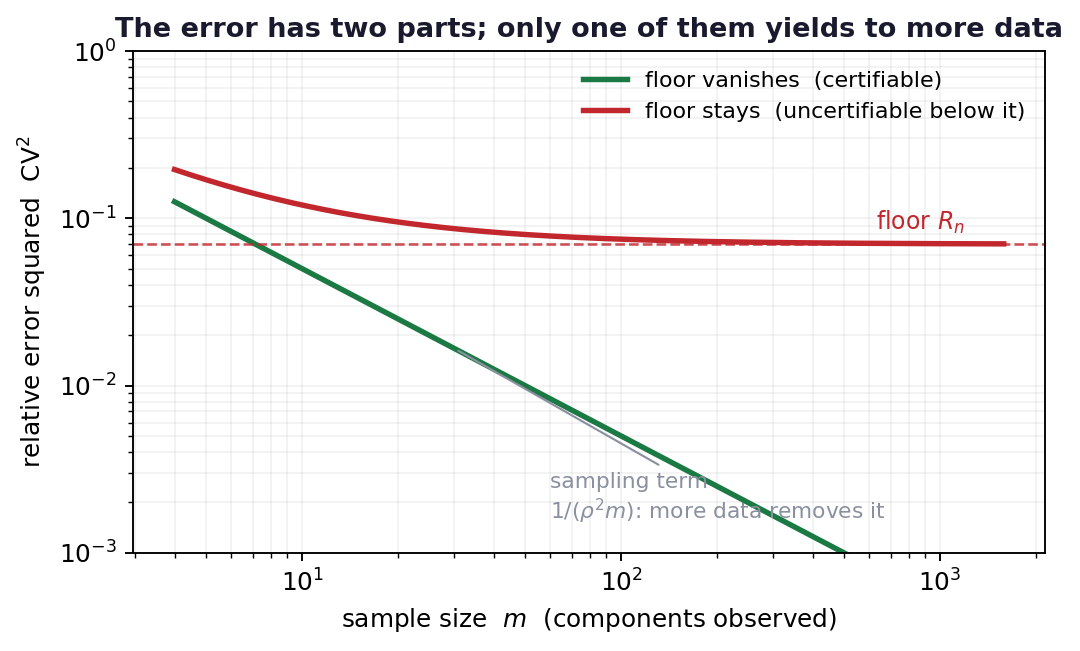
\includegraphics[width=0.66\textwidth]{fig_decomposition.png}
\caption{The estimator error (schematic, representative constants) splits into a sampling term that vanishes as $1/m$ and a floor $\Rn$ that does not. When $\chi_n=O(1)$ the floor vanishes with system size and any tolerance is reachable; when $\chi_n=\Theta(n)$ it does not, and tolerances below $\kappa\sqrt{\Rn}$ are unreachable at any $m$.}
\label{fig:decomp}
\end{figure}
\begin{figure}[t]
\centering
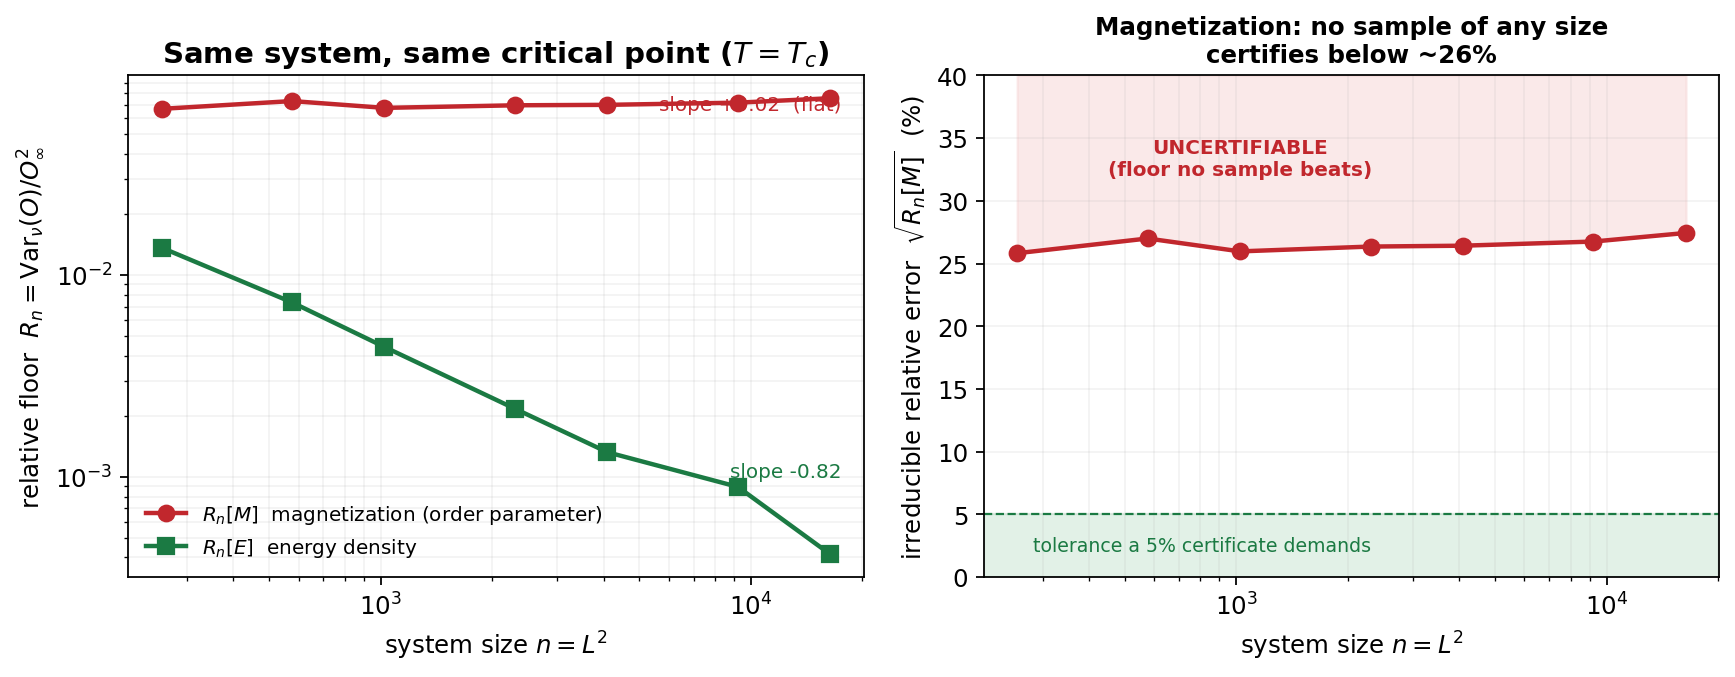
\includegraphics[width=0.99\textwidth]{fig_criticality.png}
\caption{Measured relative floor at $T_c$ (Wolff sampler, $L\le128$, bootstrap-CI slopes, two-start equilibration). \textbf{Left:} $\Rn[E]$ vanishes ($\propto n^{-0.82}$) while $\Rn[|M|]$ is flat. \textbf{Right:} the magnetisation's irreducible relative error near $26\%$ at all sizes. The recovered exponent $a[M]=0.889$ (CI $[0.869,0.908]$) reproduces the universality value $7/8$.}
\label{fig:crit}
\end{figure}

\bibliographystyle{apalike}
\bibliography{references}

\end{document}
